\pdfvariable minorversion=7
\pdfvariable inclusioncopyfonts=1

\documentclass{arialFHGR} % use either arialFHGR or timesFHGR
\newcommand{\haupttitel}{Titel der Studienarbeit}
\newcommand{\untertitel}{Untertitel}
\newcommand{\zusammenfassung}{Abstract}
\newcommand{\autorenschaft}{Max Mustermann}
\newcommand{\studiengang}{BSc Information Science}
\newcommand{\matrikelnummer}{00-000-000}
\newcommand{\adresse}{Musterstrasse 1}
\newcommand{\ort}{Musterhausen}
\newcommand{\plz}{0000}
\newcommand{\department}{[Departement]}
\newcommand{\institute}{[Institutsname]}
\newcommand{\modul}{WIAGRU}
\newcommand{\email}{max.mustermann@stud.fhgr.ch}
\newcommand{\refe}{Prof. Dr. Eva Mustermann}
\newcommand{\coRefe}{Julian Junke}
\newcommand{\abgabedatum}{01.10.1963}
\newcommand{\abgabedatumRFC}{1963-10-01}
\newcommand{\sprache}{de}
\newcommand{\schlagworte}{Keyword 1, Keyword 2}

\usepackage{setspace, fancyhdr, lscape, floatrow, caption, inputenc, graphicx, enumitem, tabularx, colorprofiles, xstring, hyphenat, chngcntr, xspace, listings, pdfpages}

\usepackage[left=3cm,right=2.5cm,top=2.5cm,bottom=2cm]{geometry}
\usepackage[backend=biber,style=apa,citestyle=apa]{biblatex}
\usepackage[autostyle]{csquotes}
\usepackage[english, nswissgerman]{babel}
\usepackage[titles]{tocloft}
\usepackage[hang,flushmargin]{footmisc}

% Settings for glossary
\usepackage[acronym,toc=true,xindy,nopostdot=true,nonumberlist,nogroupskip=true]{glossaries}
\loadglsentries{content/01_vorspann/01.4_abkuerzungsverzeichnis_glossar}
\setglossarystyle{alttree}
\setglossarypreamble[acronym]{\vspace*{-8pt}}
\makeglossaries
\glsaddall
\glsfindwidesttoplevelname

\graphicspath{{content/00_assets}} % Set path as default for including graphics
\addbibresource{content/00_assets/quellen.bib} % Add bibliography entries

% cite with acronym. 
% Example input: \citeAbbr{schweizerische_archivdirektorinnen-_und_archivdirektorenkonferenz_informations-_2018}{adk}
\newcommand{\parenciteabbr}[2]{(\acrlong{#2} [\acrshort{#2}], \citeyear{#1})}
\newcommand{\textciteabbr}[2]{\acrlong{#2} (\acrshort{#2}, \citeyear{#1})}
\newcommand{\acrfullSqBr}[1]{\acrlong{#1} [\acrshort{#1}]}

\setmonofont{Courier New}

% Settings for listings
\lstdefinestyle{codeStyle}{
    belowcaptionskip=6pt,
    belowskip=3pt,
    breaklines=true,
    numbers=left,
    basicstyle=\footnotesize\ttfamily,
    extendedchars=true,
    frame=single,
    captionpos=t,
    numberbychapter=false,
    xleftmargin=4pt,
    xrightmargin=4pt
}
\lstset{style=codeStyle}

% Settings for blockquote
\SetBlockEnvironment{quotation}
\patchcmd{\quotation}{\rightmargin}{\leftmargin 1.3cm \rightmargin 0}{}{}
\NewCommandCopy{\oldblockquote}{\blockquote}
\renewcommand{\blockquote}[1]{\oldblockquote{\noindent #1}}

% Settings for figure and table
\counterwithout{figure}{chapter}
\counterwithout{table}{chapter}

\floatsetup[figure]{
    capposition=above,
    captionskip=2pt
}

\DeclareCaptionLabelFormat{figTitle}{%
    Abbildung \the\numexpr\value{figure}\relax\\
}

\captionsetup[figure]{
    font={normalsize,stretch=1.0},
    labelfont=bf,
    labelsep=none,
    labelformat=figTitle,
    textfont=it,
    justification=raggedright,
    singlelinecheck=false,
    position=above,
}

\floatsetup[table]{
    capposition=above,
    captionskip=2pt
}

\DeclareCaptionLabelFormat{tabTitle}{%
    Tabelle \the\numexpr\value{table}\relax \\
} 

\captionsetup[table]{
    font={normalsize,stretch=1.0},
    labelfont={bf},
    labelsep=none,
    labelformat=tabTitle,
    textfont=it,
    justification=raggedright,
    singlelinecheck=false,
    position=above
}

\floatsetup[lstlisting]{
    capposition=above,
    captionskip=2pt
}

\DeclareCaptionLabelFormat{codeTitle}{%
    Programmcode \the\numexpr\value{lstlisting}\relax \\
} 

\captionsetup[lstlisting]{
    font={normalsize,stretch=1.0},
    labelfont={bf},
    labelsep=none,
    labelformat=codeTitle,
    textfont=it,
    justification=raggedright,
    singlelinecheck=false,
    position=above
}

\renewcommand{\thetable}{\arabic{table}}
\renewcommand{\thefigure}{\arabic{figure}}

% Einstellungen für tocloft / Settings for tocloft
\renewcommand{\cftfigpresnum}{Abb.~}
\renewcommand{\cfttabpresnum}{Tab.~}
\renewcommand{\cftfigaftersnum}{:}
\renewcommand{\cfttabaftersnum}{:}
\setlength{\cftfignumwidth}{2cm}
\setlength{\cfttabnumwidth}{2cm}
\setlength{\cftfigindent}{0cm}
\setlength{\cfttabindent}{0cm}

\setstretch{1.3} % Zeilenabstand / line spacing
\renewcommand{\arraystretch}{1.3} % Zeilenabstand innerhalb von Tabellen / line spacing in tables
\setlength{\parindent}{1.3cm} % Einzug neuer Absatz / Indentation new paragraph
\fancyhf{}
\renewcommand{\headrulewidth}{0pt}
\pagestyle{fancyplain}
\rfoot{\footnotesize\thepage}

\usepackage[pdfa]{hyperref}
\usepackage{hyperxmp}
\usepackage{embedfile}
\pdfvariable omitcidset=1

% 
\newcommand{\chapterNoNr}[1]{%
    \chapter*{#1}
    \addcontentsline{toc}{chapter}{#1} %
}%

\newcommand{\note}[1]{%
    \doublespacing\raggedright\footnotesize{\textit{Anmerkung:} #1}
}%

\newcommand{\sic}{%
    [\textit{sic}]\xspace
}%

\makeatletter
\def\l@lstlisting#1#2{\@dottedtocline{1}{0em}{2em}{Programmcode #1}{#2}}
\makeatother

\hypersetup{%
    pdflang=\sprache,
    pdftitle={\haupttitel},
    pdfsubtitle={\untertitel},
    pdfauthor={\autorenschaft},
    pdfdate={\abgabedatumRFC},
    pdfsubject={\zusammenfassung},
    pdfkeywords={\modul, \schlagworte},
    pdfcontactaddress={\adresse},
    pdfcontactcity={\ort},
    pdfcontactpostcode={\plz},
    pdfcontactemail={\email},
    colorlinks,
    unicode,
    allcolors=black,
    pdfapart=2,
    pdfaconformance=U
}

% 
\immediate\pdfobj stream attr{/N 3} file{sRGB.icc}
\pdfcatalog{%
  /OutputIntents [
    <<
      /Type /OutputIntent
      /S /GTS_PDFA1
      /DestOutputProfile \the\pdflastobj\space 0 R
      /OutputConditionIdentifier (sRGB)
      /Info (sRGB)
    >>
  ]
}

\begin{document}

    \renewcommand{\contentsname}{Inhaltsverzeichnis}
    \renewcommand{\listfigurename}{Abbildungsverzeichnis}
    \renewcommand{\listtablename}{Tabellenverzeichnis}
    \renewcommand{\acronymname}{Abkürzungsverzeichnis}
    \renewcommand{\lstlistlistingname}{\texorpdfstring{Programmcodeverzeichnis\bigskip}{Programmcodeverzeichnis}}
    
    % Start Vorspann
    
    \pagenumbering{Roman} % Begin roman pagenumbering

    % Titelblatt für eine Studienarbeit
     \begin{titlepage}
    
    \begin{center}
        Fachhochschule Graubünden, \institute \\
        \vspace{30mm}
        \huge\textbf{\haupttitel}\\
        \hfill \break
        \large{(\untertitel)}
    \end{center}
    
    \vfill
    
    \begin{flushleft}
    Name: \autorenschaft\\
    Studiengang: \studiengang\\
    Matrikelnr.: \matrikelnummer\\
    Adresse: \adresse, \plz~\ort\\
    E-Mail: \email\\
    ~\\
    Modul: \modul\\
    Referent/in: \refe\\
    Koreferent/in: \coRefe\\
    ~\\
    Abgabedatum: \abgabedatum
    \end{flushleft}
    
    \vspace{20mm}
    
\end{titlepage}

    % ODER für eine Abschlussarbeit
    % \begin{titlepage}
    \begin{center}
        {\large
            {\Large\textbf{\haupttitel}} \\
            \textit{\untertitel} \\
            ~\\
            An der Fachhochschule Graubünden \\
            \department \\
            \institute \\
            \vspace{2mm}
            im Studiengang \studiengang{} eingereichte \\
            ~\\
            {\Huge\textbf{Bachelorarbeit}} \\
            ~\\
            zur Erlangung des akademischen Grades \\
            eines Bachelor of Science (B.Sc.)
    
            \vspace{40mm}
            vorgelegt von \\
            \vspace{4mm}
            {\Large\textbf{\autorenschaft}} \\
            \vspace{4mm}
            Matrikelnr.: \matrikelnummer \\
            E-Mail: \email \\
            ~\\~\\
            Erstgutachter/in: \refe \\
            Zweitgutachter/in: \coRefe \\
            ~\\
            Eingereicht am: \abgabedatum
        } % end large
    \end{center}
\end{titlepage}


    \chapter*{Abstract}
Sit amet mattis vulputate enim nulla aliquet. Risus at ultrices mi tempus imperdiet nulla malesuada pellentesque. Turpis nunc eget lorem dolor sed viverra ipsum nunc aliquet. Turpis egestas integer eget aliquet nibh praesent. Sed euismod nisi porta lorem mollis aliquam ut porttitor leo. Sem viverra aliquet eget sit. Id leo in vitae turpis massa sed elementum tempus egestas. Pharetra vel turpis nunc eget lorem dolor sed viverra ipsum. Velit ut tortor pretium viverra suspendisse potenti nullam ac. Eget sit amet tellus cras adipiscing enim eu turpis. Pulvinar neque laoreet suspendisse interdum consectetur libero. Consequat interdum varius sit amet mattis vulputate enim nulla aliquet. Amet purus gravida quis blandit turpis cursus in hac habitasse. In aliquam sem fringilla ut morbi tincidunt augue. Tellus molestie nunc non blandit massa enim nec. Mi eget mauris pharetra et ultrices neque.


    \tableofcontents % Inhaltsverzeichnis
        
    % List of figures
    \cleardoublepage
    \phantomsection
    \addcontentsline{toc}{chapter}{\listfigurename}
    \listoffigures
    
    % List of tables
    \cleardoublepage
    \phantomsection
    \addcontentsline{toc}{chapter}{\listtablename}
    \listoftables

    % List of acronyms
    \printglossary[type=\acronymtype]
    \cleardoublepage
    \newpage
    % Ende Vorspann
    
    % Start Textteil
    \pagenumbering{arabic} % Begin arabic pagenumbering
    \chapter{Einleitung}
Das ist die Einleitung. Interssantes findest du aber eher im Kapitel \ref{kap:eins}.
    \chapter{Forschungsproblem}
\label{kap:forschungsproblem_forschungsziel}
Schweizer fahren gerne Zug, dies zeigt ein Artikel von Litra, welcher die Nutzung des Zuges in Europa untersucht untersuchte \parencite{litra_bahnfahrtstatistik_europa_2023}. Alleine im Jahr 2023 legten die Schweizer rund 2'466 Bahnkilometer pro Einwohner zurück (siehe Abbildung \ref{fig_schweizer_fahren_zug}. Dies entspricht einem Zuwachs von rund 13 Prozent im Vergleich zum Vorjahr. 

\begin{figure}[H]
    \caption{Zurückgelegte Kilometer pro Einwohnerin und Einwohner 2023 (Personenkilometer) \parencite{litra_bahnfahrtstatistik_europa_2023}}
    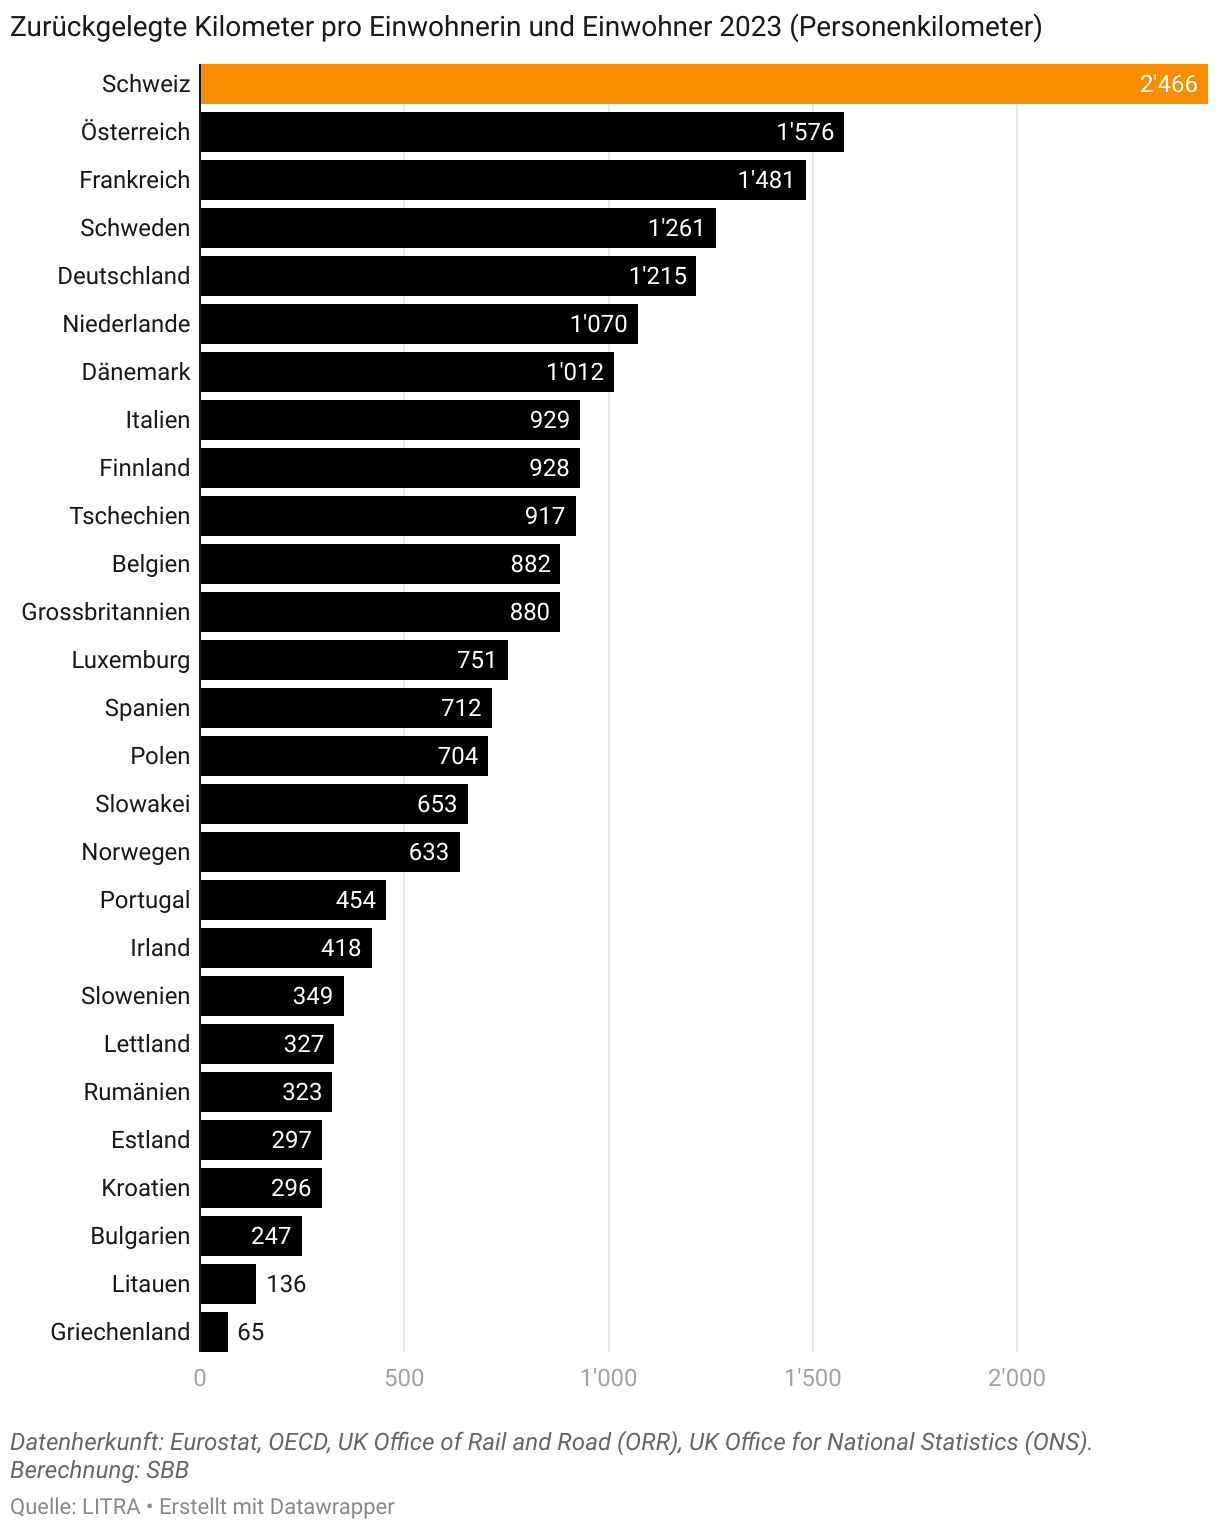
\includegraphics[width=.4\linewidth]{content/00_assets/schweizer_fahren_zug.png}
    \label{fig_schweizer_fahren_zug}
\end{figure}

Auch scheint es keine Anzeichen einer Abschwächung der Zugnutzung zu geben, ganz im Gegenteil. Gemäss der \acrfull{sbb} sollen im Jahr 2040 bereits zwei Millionen Menschen pro Tag mit dem Zug fahren, dies entspricht einer Zunahme von rund 30 Prozent \parencite{sbb_ausbauschritt_2025}.

Schaut man sich die Zahlen und Fakten für das SBB-Zugverkehrsnetz aus dem Jahr 2024 an, ergeben sich auch beachtliche Werte. Täglich werden rund 1.4 Millionen Menschen mithilfe von 11'569 Zügen transportiert. Um das Zugnetz der SBB auf Stand zu halten, werden rund 20'000 Baustellen pro Jahr betrieben. Um es mit den Worten der SBB auszudrücken, ist Bauen und Fahren eine Herausforderung \parencite[S.8 - 9]{sbb_geschäftsbericht_2024}. Jedoch ist insbesondere das Fahren nicht nur eine Herausforderung für die Zugnetzbetreiber, sondern auch für die Passagiere, primär dann, wenn Verspätungen involviert sind.

Die vorliegende Arbeit hat sich daher zum Ziel gesetzt, visuelle Muster und Anomalien im SBB-Zugverkehrsnetz zu analysieren. Hierzu soll ein webbasiertes Visual-Analytics-Tool entworfen werden. Im Fokus der Arbeit stehen hierbei primär Zugverspätungen. Nebst der eigentlichen Visualisierung der Daten stehen vor allem Algorithmen im Zentrum. Diese sollen dabei helfen, visuelle Muster auf anschauliche Weise zugänglich zu machen.


    \chapter{Literaturübersicht}
\label{kap:literaturübersicht}
Die nachfolgende Literaturübersicht bietet einen Überblick über relevante Projekte und Visualisierungen, welche sich mit Zugverspätungen und deren Auswirkungen auf ein Zugnetzwerk befassen. Nebst den visuellen werden auch die algorithmischen Verfahren, insbesondere zur Erkennung von Mustern, betrachtet.

\section{Visualisierungs-Pipeline}
\textbf{Dashboards} sind ein effektives Werkzeug, um grosse Mengen an Daten verständlich und auf einen Blick darzustellen. Um ein qualitativ hochwertiges Dashboard zu erstellen, müssen sowohl die Daten und Algorithmen als auch die Visualisierungen und Interaktionen aufeinander abgestimmt sein. Um das Zusammenspiel dieser Komponenten zu veranschaulichen, werden häufig \textbf{Visualisierungs-Pipelines} verwendet (siehe Abbildung \ref{fig_pipeline_traffic_visualization}).

\begin{figure}[H]
    \caption{Visualisierungspipeline für Verkehrsdaten \parencite[S. 2971]{survey_traffic_data_visualization_2015}}
    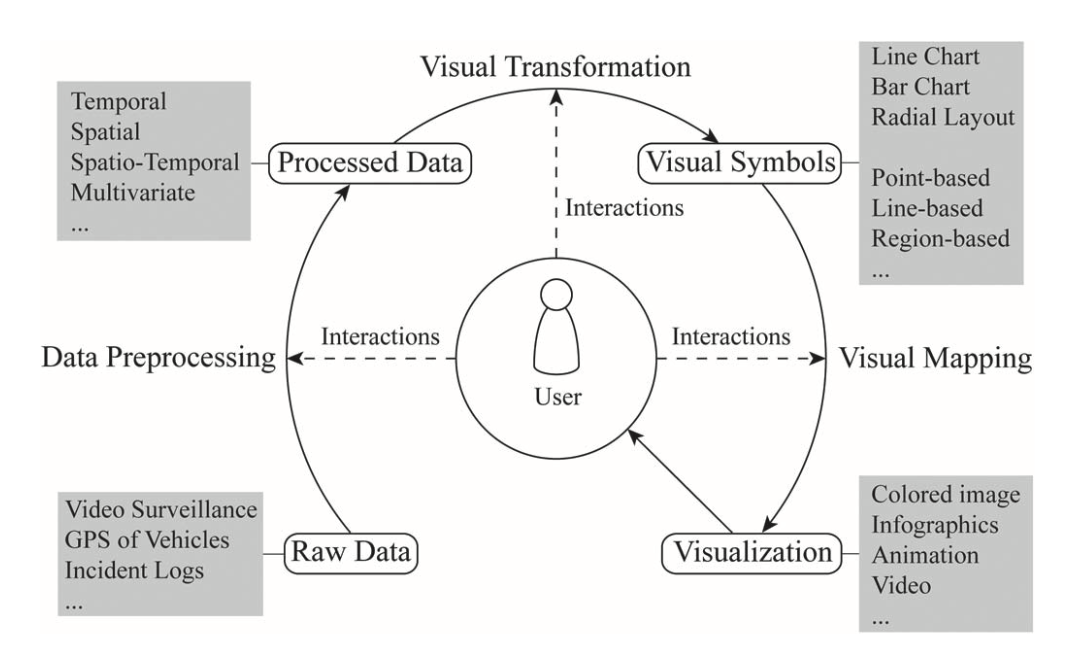
\includegraphics[width=.8\linewidth]{content/00_assets/traffic_visualization_pipeline.png}
    \label{fig_pipeline_traffic_visualization}
\end{figure}

Das Paper von Chen et al. betrachtet verschiedene Visualisierungen zum Thema Verkehrsdaten anhand einer solchen Pipeline. Eine Visualisierung über Verkehrsdaten durchläuft gemäss Chen et al. vier verschiedene Phasen. In der Phase \textit{Raw Data} werden die Daten erfasst. Dies geschieht meist über Sensoren, GPS oder Log-Aufzeichnungen der Geräte. Anschliessend werden die Daten in der \textit{Data Preprocessing} Phase aufbereitet. Im Rahmen des Data Preprocessing werden zudem Datenfehler und Ausreisser entfernt. Aufgrund der grossen Datenmengen, welche bei Verkehrsdaten auftreten, ist es wichtig, dass diese Daten effizient gespeichert werden. Dies geschieht über \textit{Datenaggregationen} und die richtige Wahl eines effizienten \textit{Datenverwaltungssystems}. Das Ergebnis des Data Preprocessing ist ein Datensatz mit sowohl räumlichen, zeitlichen als auch multivariaten Informationen. Durch \textit{Visual Symbols} werden die Daten dem Nutzer mithilfe von unterschiedlichen Visualisierungen (bspw. Liniendiagramm) dargestellt. Um das Verständnis der Daten noch weiter zu fördern, werden im Schritt \textit{Visual Mapping} visuelle Variablen verwendet \parencite[S.2971]{survey_traffic_data_visualization_2015}. Ein Beispiel für die Verwendung von visuellen Variablen ist das Projekt \textit{Trains in Time} (siehe Abbildung \ref{fig_trains_in_time}). Hier werden die visuellen Variablen Grösse und Farbe verwendet, um die Zugverspätung und Zugauslastung im Pariser Streckennetz zu visualisieren. Die Farbe repräsentiert hierbei die Verspätung und die Grösse der Kreise die Auslastung eines Zuges \parencite{trains_of_data_2012}.   

\begin{figure}[H]
    \caption{Trains in Time \parencite{trains_of_data_2012}}
    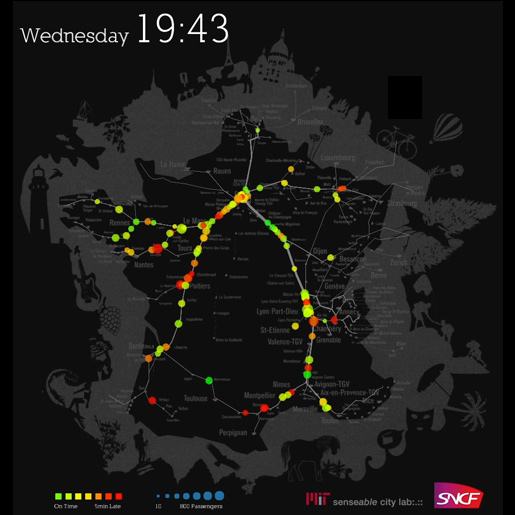
\includegraphics[width=.5\linewidth]{content/00_assets/trains_in_time.jpg}
    \label{fig_trains_in_time}
\end{figure}

Ein weiteres Beispiel für die Verwendung von visuellen Variablen ist das Dashboard von Dimanche et al. (siehe Abbildung \ref{fig_massive_railway_visualization}). Dieses Dashboard richtet sich primär an Experten und erlaubt es, das Pariser Zugverkehrsnetzwerk zu explorieren. Die Züge werden hierbei als Rechtecke visualisiert. Die Breite des Rechtecks entspricht der Fahrzeit, die Länge entspricht der zurückgelegten Strecke und die Farbe widerspiegelt die Verspätung \parencite{visualization_tool_operating_experts_2017}.

\begin{figure}[H]
    \caption{Visualisierung von einzelnen Zügen und deren Verspätungen \parencite[S. 15843]{visualization_tool_operating_experts_2017}}
    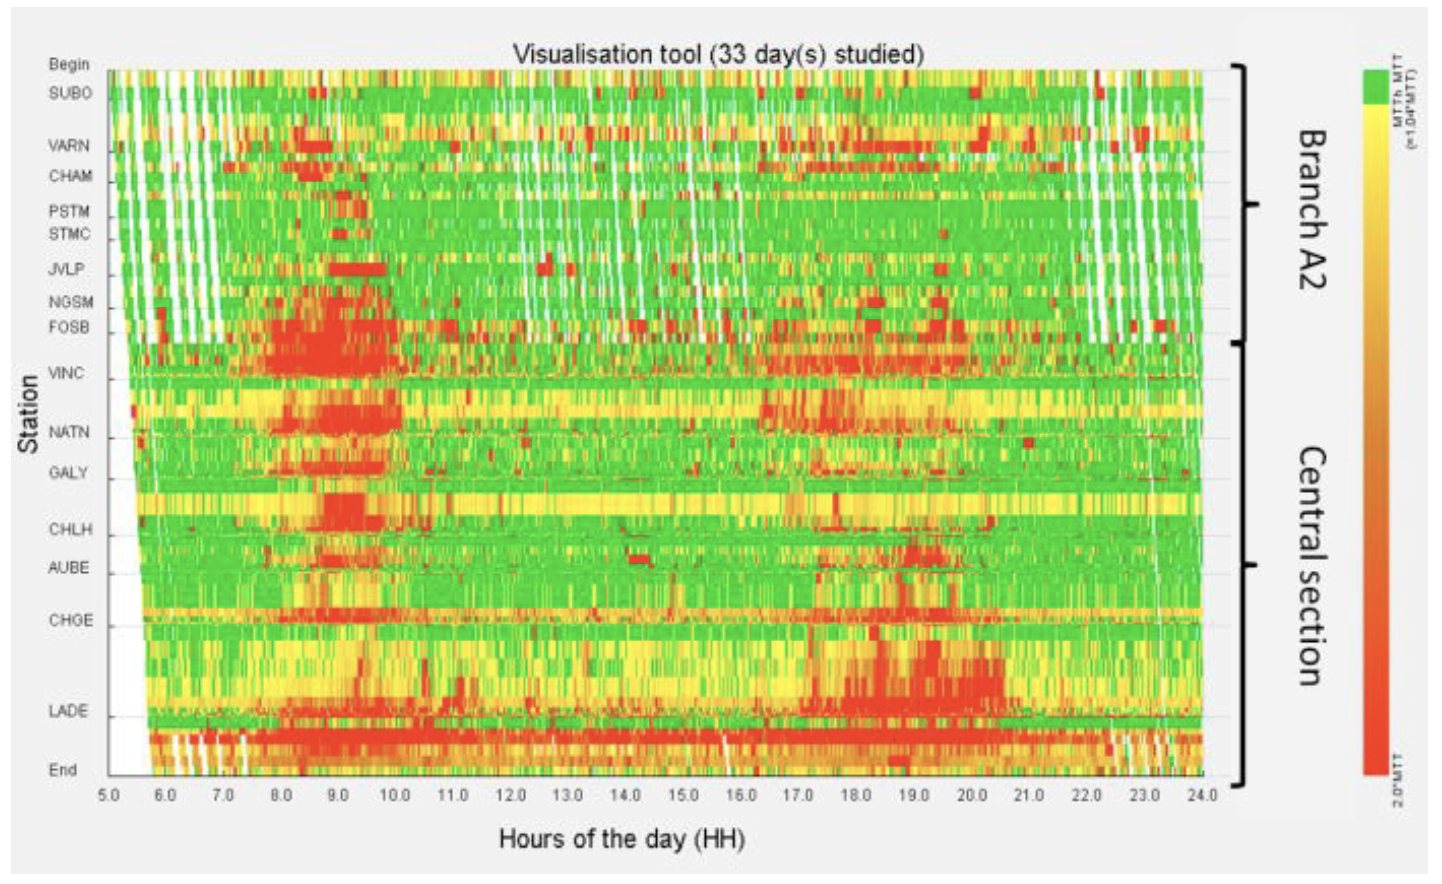
\includegraphics[width=.5\linewidth]{content/00_assets/massive_railway_visualization.png}
    \label{fig_massive_railway_visualization}
\end{figure}

Die Visualisierungs-Pipeline ist ein wiederkehrender Zyklus, worin der Nutzer mithilfe von Interaktionen Einfluss auf diverse Aspekte dieses Zyklus nehmen kann. Durch Filtereinstellungen wird die Datenmenge beeinflusst. Mithilfe von Parametern kann direkter Einfluss auf die Funktionsweise der dahinterliegenden Algorithmen genommen werden\parencite[S.2971]{survey_traffic_data_visualization_2015}.

\section{Dashboard Visualisierungen}
Wie bereits angesprochen sind Dashboards eine beliebte Option, um komplexe und grosse Datenmengen zu visualisieren. Ein Dashboard erlaubt es, unterschiedliche Sichten auf den gleichen Datensatz zu erhalten. Dies geschieht mithilfe von unterschiedlichen Visualisierungen. Jede Visualisierung veranschaulicht hierbei einen anderen Aspekt der Daten. Visualisierungen sind keine Momentaufnahme, sondern interaktive Sichten auf Daten. Der Nutzer kann mittels diverser Einstellungen (Filtereinstellungen, Parameter etc.) Einfluss auf das finale Aussehen einer Visualisierung nehmen. Auch können die Visualisierungen mithilfe von Brushing und Linking Verfahren «verbunden» werden. 

Ein Beispiel für ein Dashboard, welches unterschiedliche Sichten ermöglicht, ist das Dashboard von Jeph et al. (siehe Abbildung \ref{fig_raildash}). Ihr Dashboard visualisiert den Einfluss von Ereignissen auf den Zugverkehr in Tokyo sowie auf das Laufverhalten von einzelnen Personen. Hierbei wurden grosse Mengen von Smartphone-GPS-Daten, Daten über Ereignisse und Events, sowie Zugnetzwerkdaten kombiniert \parencite{raildash_2022}.

\begin{figure}[H]
    \caption{Raildash Dashboard \parencite[S. 93]{raildash_2022}}
    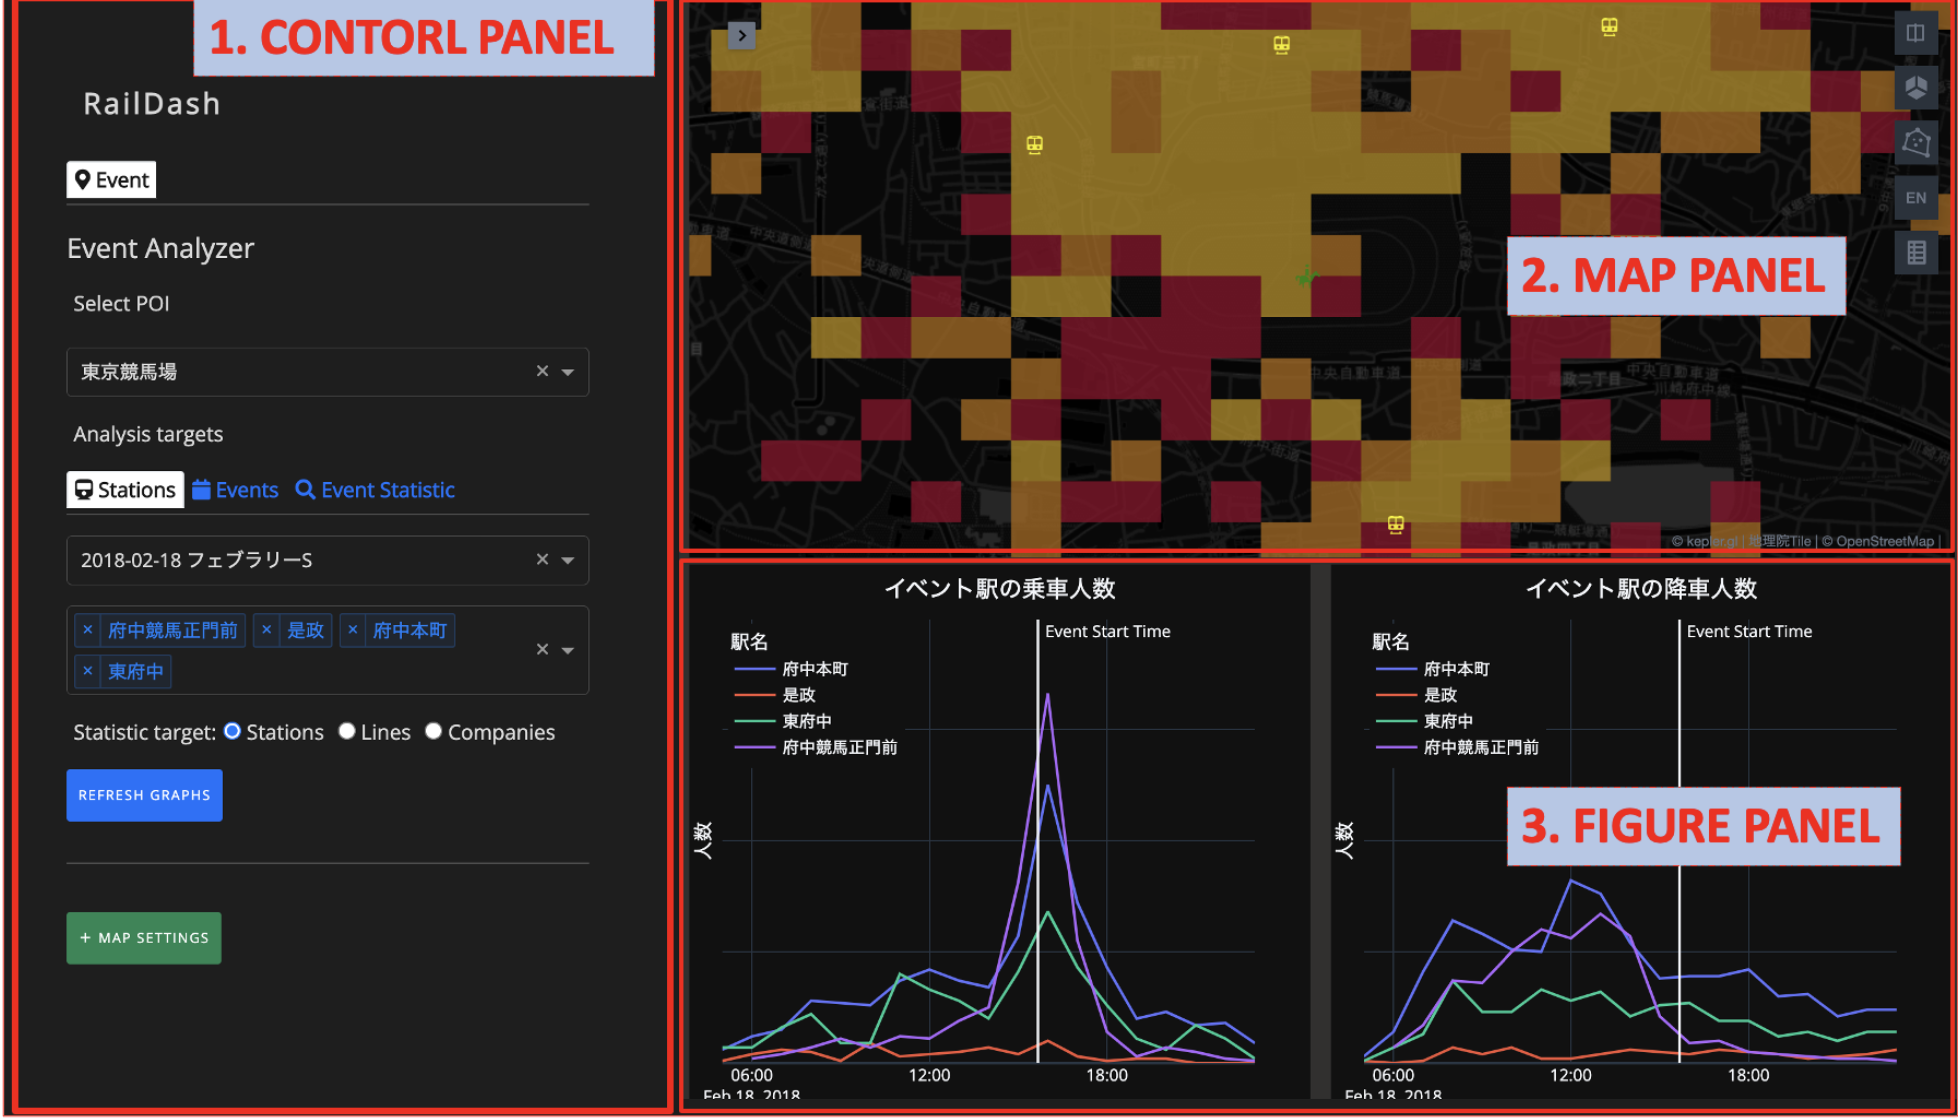
\includegraphics[width=.5\linewidth]{content/00_assets/raildash.png}
    \label{fig_raildash}
\end{figure}

Um ein qualitativ hochwertiges Dashboard zu gestalten, gibt es diverse etablierte Patterns und Regeln. Zu den bekanntesten Regeln gehören die «8 goldenden Regeln» von Ben Shneidermann \parencite{golden_rules_dashboard}. Weitere zentrale Kriterien sind die Datenqualität und insbesondere die korrekte Wahl der passenden Visualisierung. Wird eine schlechte Visualisierung gewählt, resultiert dies in einem schlechten Dashboard. Es folgt daher ein Überblick über etablierte Visualisierungen und deren Anwendungsfälle, aufgezeigt anhand der zwei wichtigsten Datentypen in Verkehrsdaten, \textbf{räumliche} sowie \textbf{zeitliche} Daten. 

\subsection{Zeitliche Visualisierungen}
Bei den \textit{zeitlichen} Daten wird gemäss Chen et al. zwischen \textbf{linearen} und \textbf{periodischen} Zeitintervallen unterschieden. \textit{Lineare Zeitintervalle} haben einen definierten Start und Endpunkt. Solche Zeitintervalle beschreiben mittels Höhen- und Tiefpunkte, wie sich die Daten über die Zeit ändern. Für lineare Zeitintervalle werden häufig Liniendiagramme verwendet. Liniendiagramme sind einfach zu interpretieren, jedoch nicht die geeignete Wahl, wenn es um die Darstellung von \textit{mehreren Variablen} geht (Visual Clutter Problematik). Nebst Liniendiagramme bieten sich auch Theme Rivers an \parencite[S. 2973]{survey_traffic_data_visualization_2015}.

\textbf{Periodische Zeitintervalle} beschreiben wiederkehrende Prozesse mit einem bestimmten Intervall (Wochentage, Monate etc.). Für solche Daten eignen sich besonders radiale Visualisierungen. In Abbildung \ref{fig_radial_layout} wird ein Tag als Kreis visualisiert, wobei die Farbe der Kreissegmente die Verkehrsauslastung darstellt \parencite[S. 2973 - 2974]{survey_traffic_data_visualization_2015}.

\begin{figure}[H]
    \caption{Radiale Visualisierung \parencite[S. 5]{radial_layout_t_watcher}}
    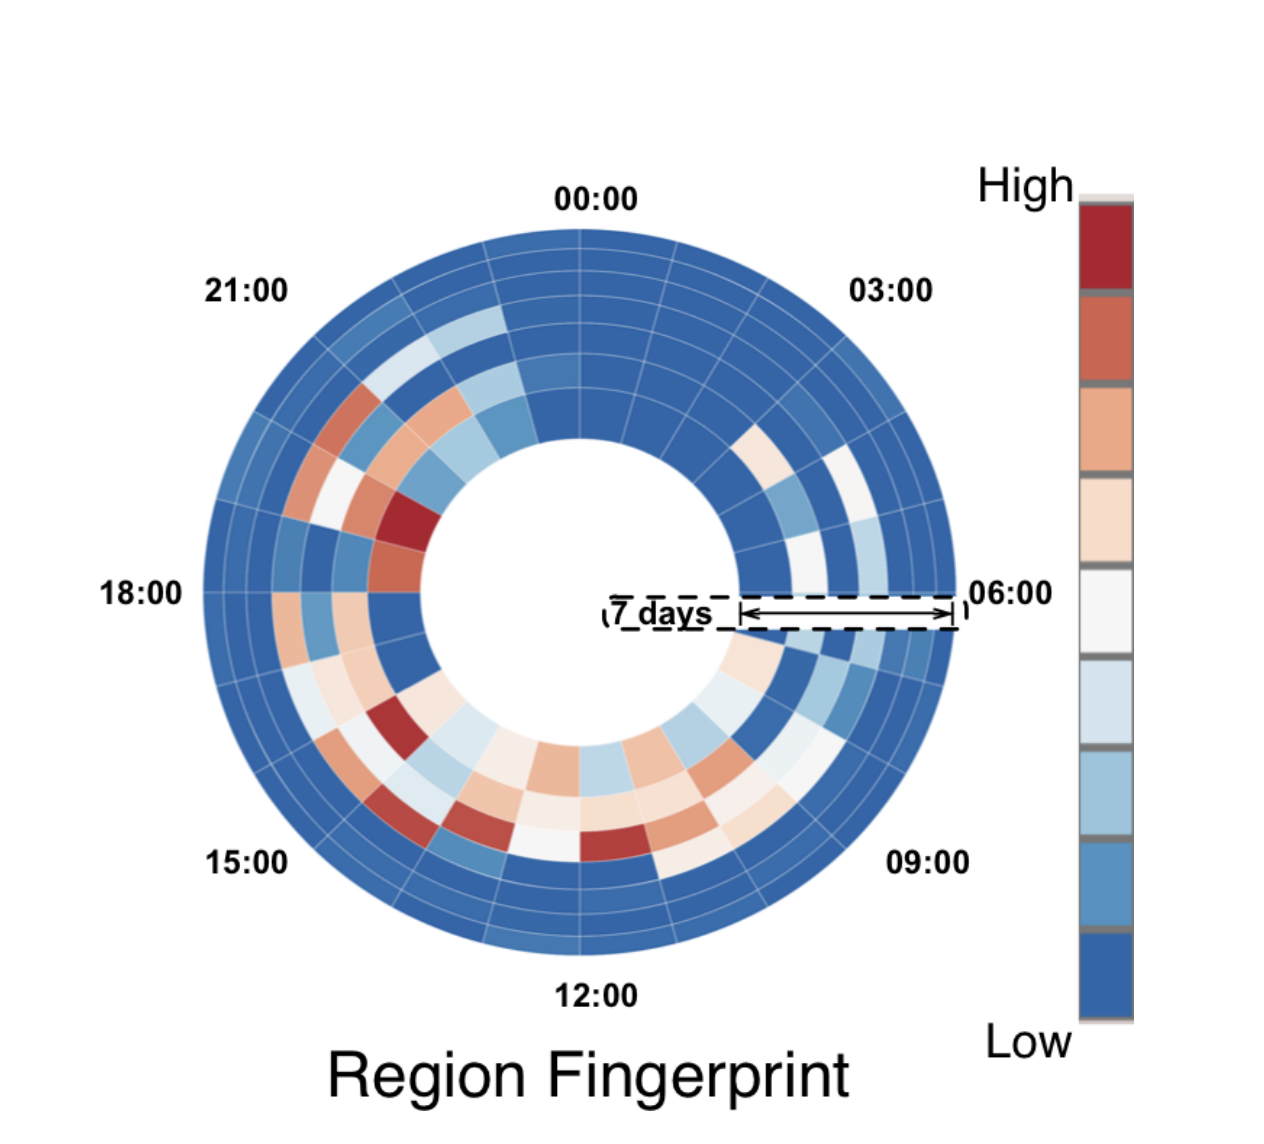
\includegraphics[width=.5\linewidth]{content/00_assets/radial_layout.png}
    \label{fig_radial_layout}
\end{figure}

\subsection{Räumliche Visualisierungen}
Räumliche Eigenschaften lassen sich gemäss Chen et al. in \textbf{punktebasierte, linienbasierte}, sowie \textbf{regionenbasierte} Visualisierungen einteilen \parencite[S. 2974 - 2975]{survey_traffic_data_visualization_2015}.

\textbf{Punktbasierte Visualisierungen} repräsentieren die Daten als Punkte. Über die visuellen Variablen Grösse und Farbe können dem Nutzer weitere Aspekte vermittelt werden. Der Vorteil von punktbasierten Visualisierungen besteht darin, dass der Nutzer den Zustand aller Objekte gleichzeitig beobachten kann. Zudem können Punktvisualisierungen dabei helfen, Cluster hervorzuheben. Jedoch besteht bei grossen Datenmengen die Gefahr von Visual Clutter. Eine Möglichkeit, um Visual Clutter zu vermindern, ist die Verwendung von Heatmaps in Kombination mit dem \textbf{\acrfull{kde}} Algorithmus (siehe Abbildung \ref{fig_heatmap_kde}).

\begin{figure}[H]
    \caption{Heatmap-Visualisierung mit KDE-Algorithmus \parencite{vait_system}}
    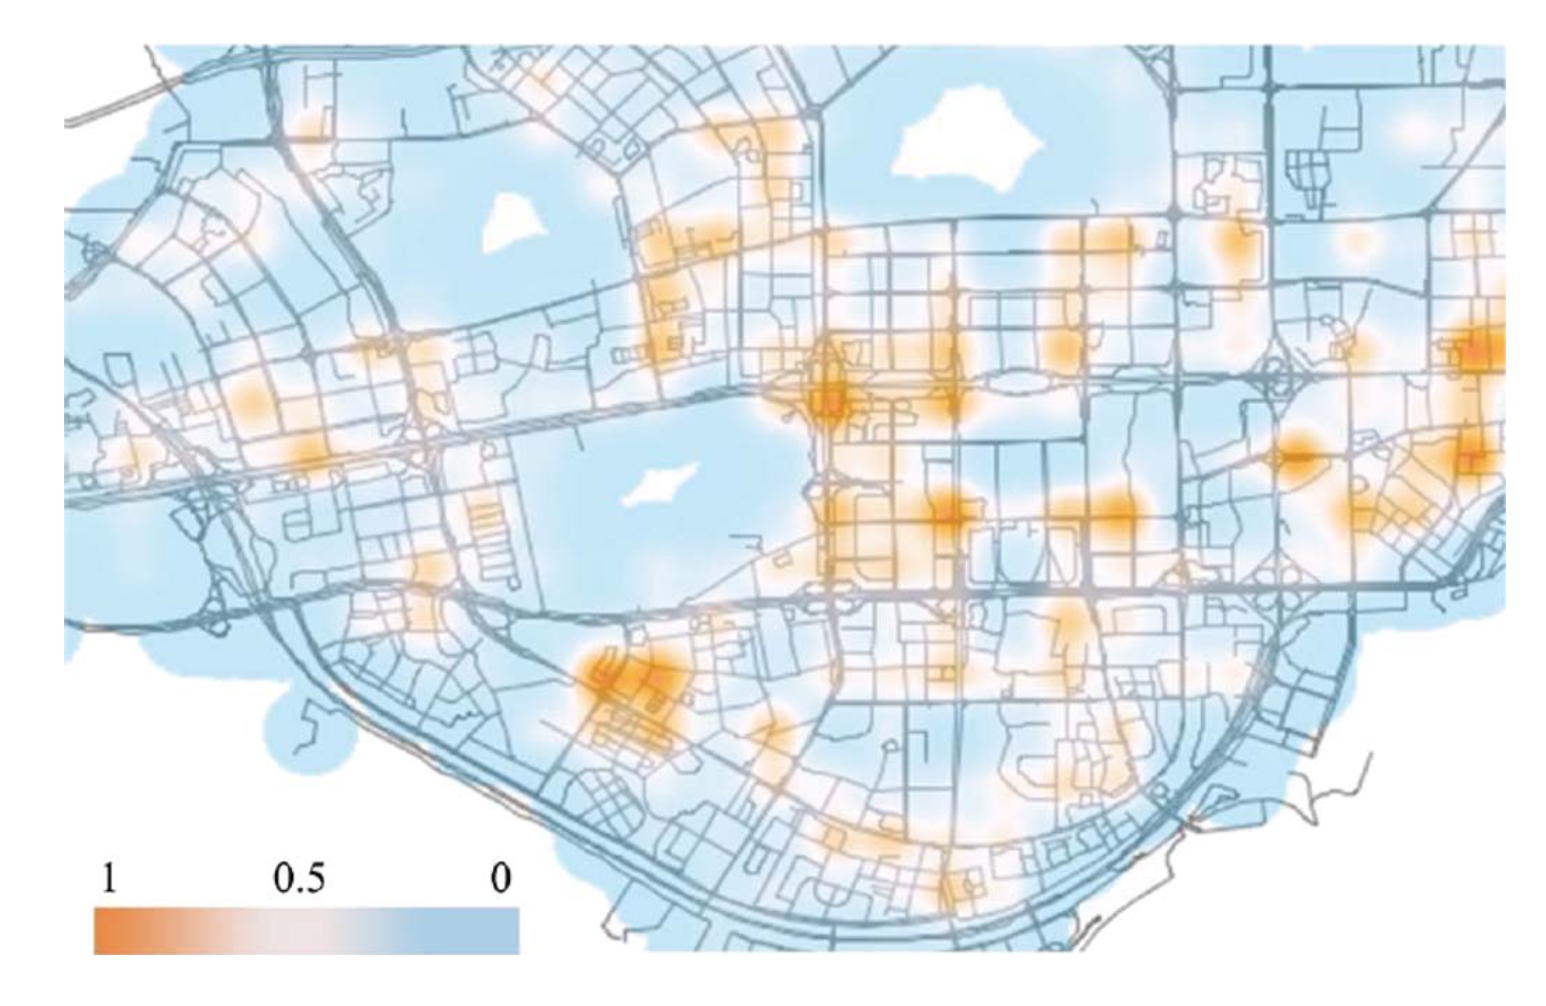
\includegraphics[width=.5\linewidth]{content/00_assets/heatmap_kde.png}
    \label{fig_heatmap_kde}
\end{figure}

\textbf{Linienbasierte Visualisierungen} werden eingesetzt, um den Fluss von Verkehrsnetzwerken zu veranschaulichen. Im Falle von Zugnetzwerken können etwa die Streckennetze als einzelne Linien (Trajektorien) dargestellt werden, wobei die Dicke der Linie die Auslastung und die Farbe die Verspätung visualisieren könnte. Bei einer grossen Anzahl von Linien entsteht jedoch auch wieder die Gefahr von Visual Clutter. Ein bewährter Lösungsansatz für dieses Problem ist das sogenannte «Edge Bundling». Hierbei werden ähnliche Linien zu einem «Bündel» zusammengefasst \parencite[S. 2974 - 2976]{survey_traffic_data_visualization_2015}. Eine weitere Möglichkeit besteht darin, anstelle von Edge Bundling den \acrshort{kde} Algorithmus auf die Trajektorien anzuwenden (siehe Abbildung \ref{fig_line_kde}).

\begin{figure}[H]
    \caption{Linienbasierte Visualisierung mit KDE-Algorithmus \parencite[S. 7]{streaming_data_kde}}
    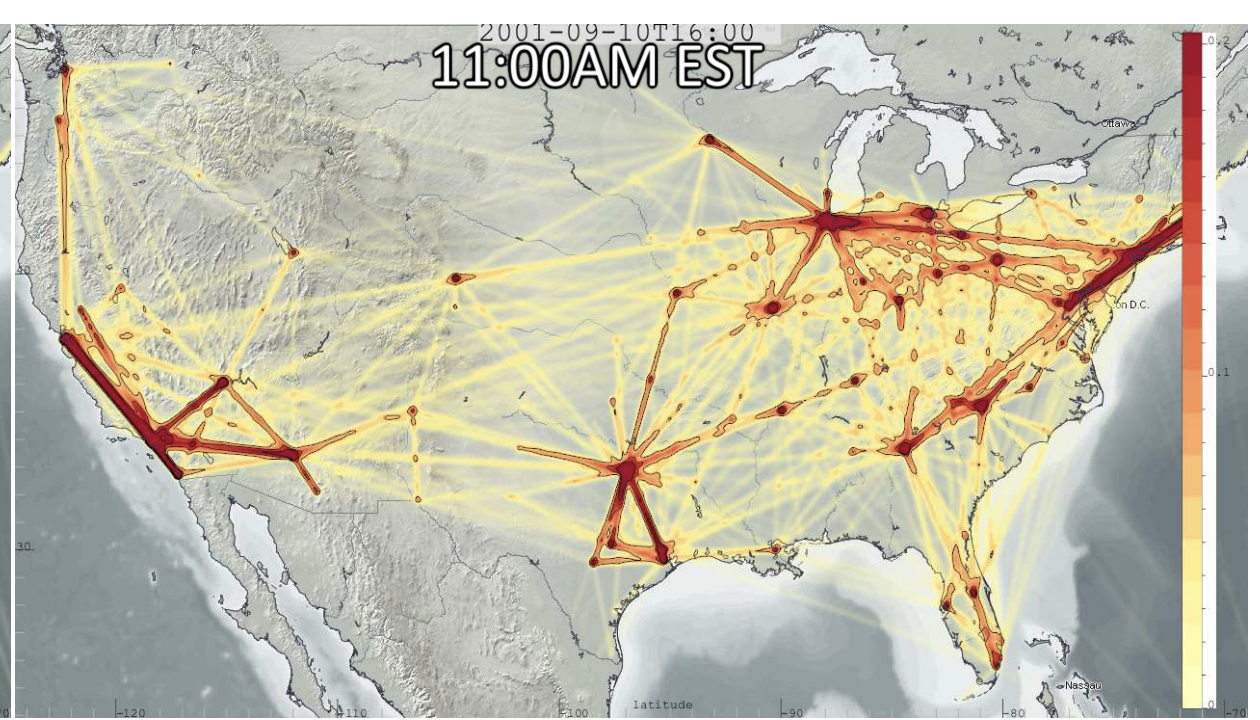
\includegraphics[width=.5\linewidth]{content/00_assets/line_visualization_kde.png}
    \label{fig_line_kde}
\end{figure}

\textbf{Regionalbasierte Visualisierungen} erlauben es gemäss Chen et al. Makro-Patterns (Zugverspätungen pro Region) in Verkehrsdaten zu visualisieren. Sie sind jedoch nicht geeignet, um Mikro-Patterns von einzelnen Zügen zu visualisieren \parencite[S. 2976]{survey_traffic_data_visualization_2015}.

\section{Erkennung von visuellen Mustern}
Nebst den bereits besprochenen Methoden wie Edge Bundling und dem \acrshort{kde} Algorithmus existieren noch andere Möglichkeiten, um visuelle Muster eines Verkehrsdatensatzes hervorzuheben. Eine bekannte Vorgehensweise aus dem Bereich Data-Mining, um visuelle Muster zu identifizieren, ist das Clustering. Lopez et al. untersuchten während 35 Tagen die Verkehrsdaten von Amsterdam. Mithilfe des K-Means, DBSCAN sowie weiterer Cluster-Algorithmen konnten sie 9 verschiedene Cluster für das Verkehrsverhalten identifizieren \parencite{lopez_2017}. Toshniwal et al. nutzten ebenfalls verschiedene Clusteralgorithmen, um Muster im Stadtverkehr von Aarthus (Dänemark) zu identifizieren. Mithilfe von Sensoren an spezifischen Ortschaften wurde die Anzahl der vorbeifahrenden Fahrzeuge ermittelt. Die Daten wurden anschliessend entsprechend aggregiert (Minuten, Stunden etc.). Für die Analyse des zeitlichen als auch räumlichen Verhaltens wurden diverse Cluster-Algorithmen verwendet. Für das \textbf{zeitliche} Verhalten wurde der DBSCAN Algorithmus verwendet. Für das \textbf{räumliche} Verhalten wurde unter anderem ein hierarchisches Clustering (Agglomerative Nesting) verwendet (siehe Abbildung \ref{fig_clustering_urban_traffic}).

\begin{figure}[H]
    \caption{Cluster-Algorithmen gemäss Toshinwal et al. \parencite[S. 1050]{clustering_urban_traffic_data}}
    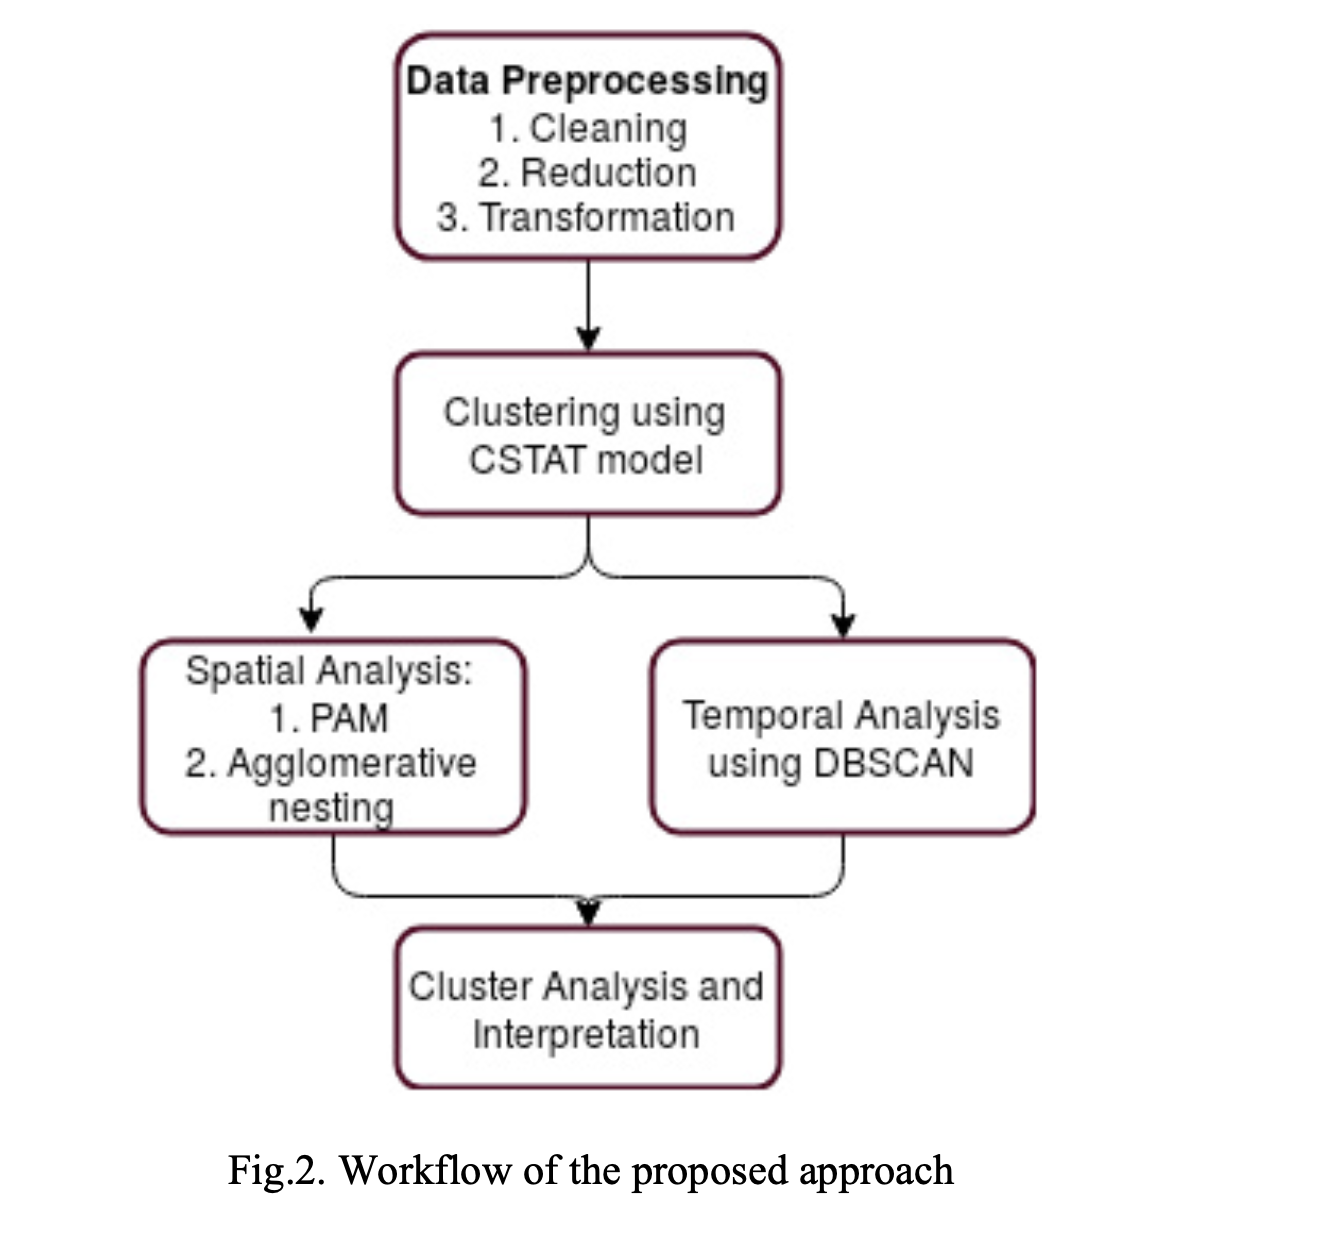
\includegraphics[width=.5\linewidth]{content/00_assets/urban_traffic_clustering_methods.png}
    \label{fig_clustering_urban_traffic}
\end{figure}

\section{Weitere Ansätze}
Selbstverständlich gibt es noch viele weitere Möglichkeiten, um Verspätungen innerhalb eines Netzwerks zu visualisieren, bspw. mithilfe von \textit{Simulationen} und \textit{Machine Learning} Verfahren. Xia et al. nutzten Deep Learning, um Verspätungen innerhalb des Zugnetzwerkes von Tokyo sowohl zu simulieren als auch vorherzusagen \parencite[S.56]{xia_2018}.


    \chapter{Forschungsfragen}
\label{kap:forschungsfragen}
Hauptfokuspunkt der Masterarbeit sind Grafstrukturen in Form von Zugverkehrsnetzwerken. Eine Grafstruktur (siehe Abbildung \ref{fig_graph_structure}) besteht aus zwei Elementen, Knoten (Vertices) und Kanten (Edges). 
\begin{figure}[H]
    \caption{Beispiel einer Grafstruktur \parencite[S. 8]{wilson_2010}}
    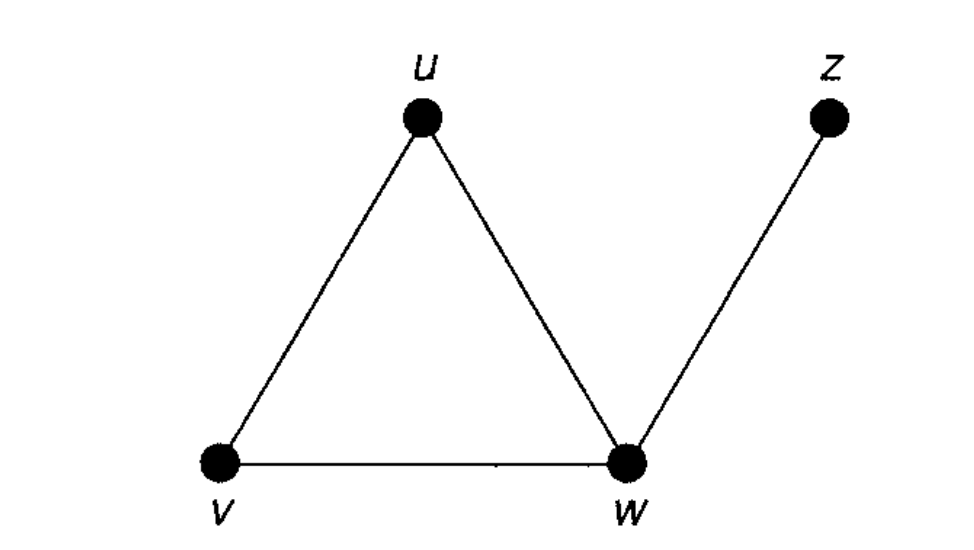
\includegraphics[width=.5\linewidth]{content/00_assets/graph_structure.png}
    \label{fig_graph_structure}
\end{figure}

Im Falle eines Zugnetzwerkes können die Knoten die einzelnen Stationen und die Kanten die Zuglinien widerspiegeln.  Es wird insbesondere das Zugverkehrsnetzwerk der \acrshort{sbb} betrachtet. Primär werden die Auswirkungen von Verspätungen auf ein solches Netzwerk analysiert. Die Hauptforschungsfrage der Arbeit lautet: 

\begin{itemize}
    \item \textbf{Welche Trends und Anomalien ergeben sich im dynamischen Zugnetzwerk der SBB?}
\end{itemize}

Abgeleitet von dieser Hauptforschungsfrage ergeben sich folgende interessante untergeordnete Fragen:

\begin{itemize}
    \item \textbf{Welche Zugstationen und Zuglinien sind am stärksten von Verspätungen betroffen und welche Clusterbildungen entstehen hieraus?}
    \item \textbf{Welche zeitlichen Muster ergeben sich pro Zuglinie und Station in Hinblick auf Verspätungen?}
\end{itemize}

    \chapter{Forschungsdesign}
\label{kap:forschungsdesign}
Das Hauptziel der Arbeit ist das Erstellen eines Visual-Analytics-Tools, mithilfe dessen Trends und Anomalien aufgrund von Verspätungen im \acrshort{sbb} Zugnetzwerk exploriert werden können. Das Vorgehen orientiert sich hierbei an der Visualisierungspipeline von Chen et al. (siehe Abbildung \ref{fig_pipeline_traffic_visualization}), fügt jedoch noch zusätzliche Schritte wie UI-Design, Algorithmen sowie Performance-Analyse hinzu (siehe Abbildung \ref{fig_vorgehen}).

\begin{figure}[H]
    \caption{Vorgehensweise (eigene Darstellung)}
    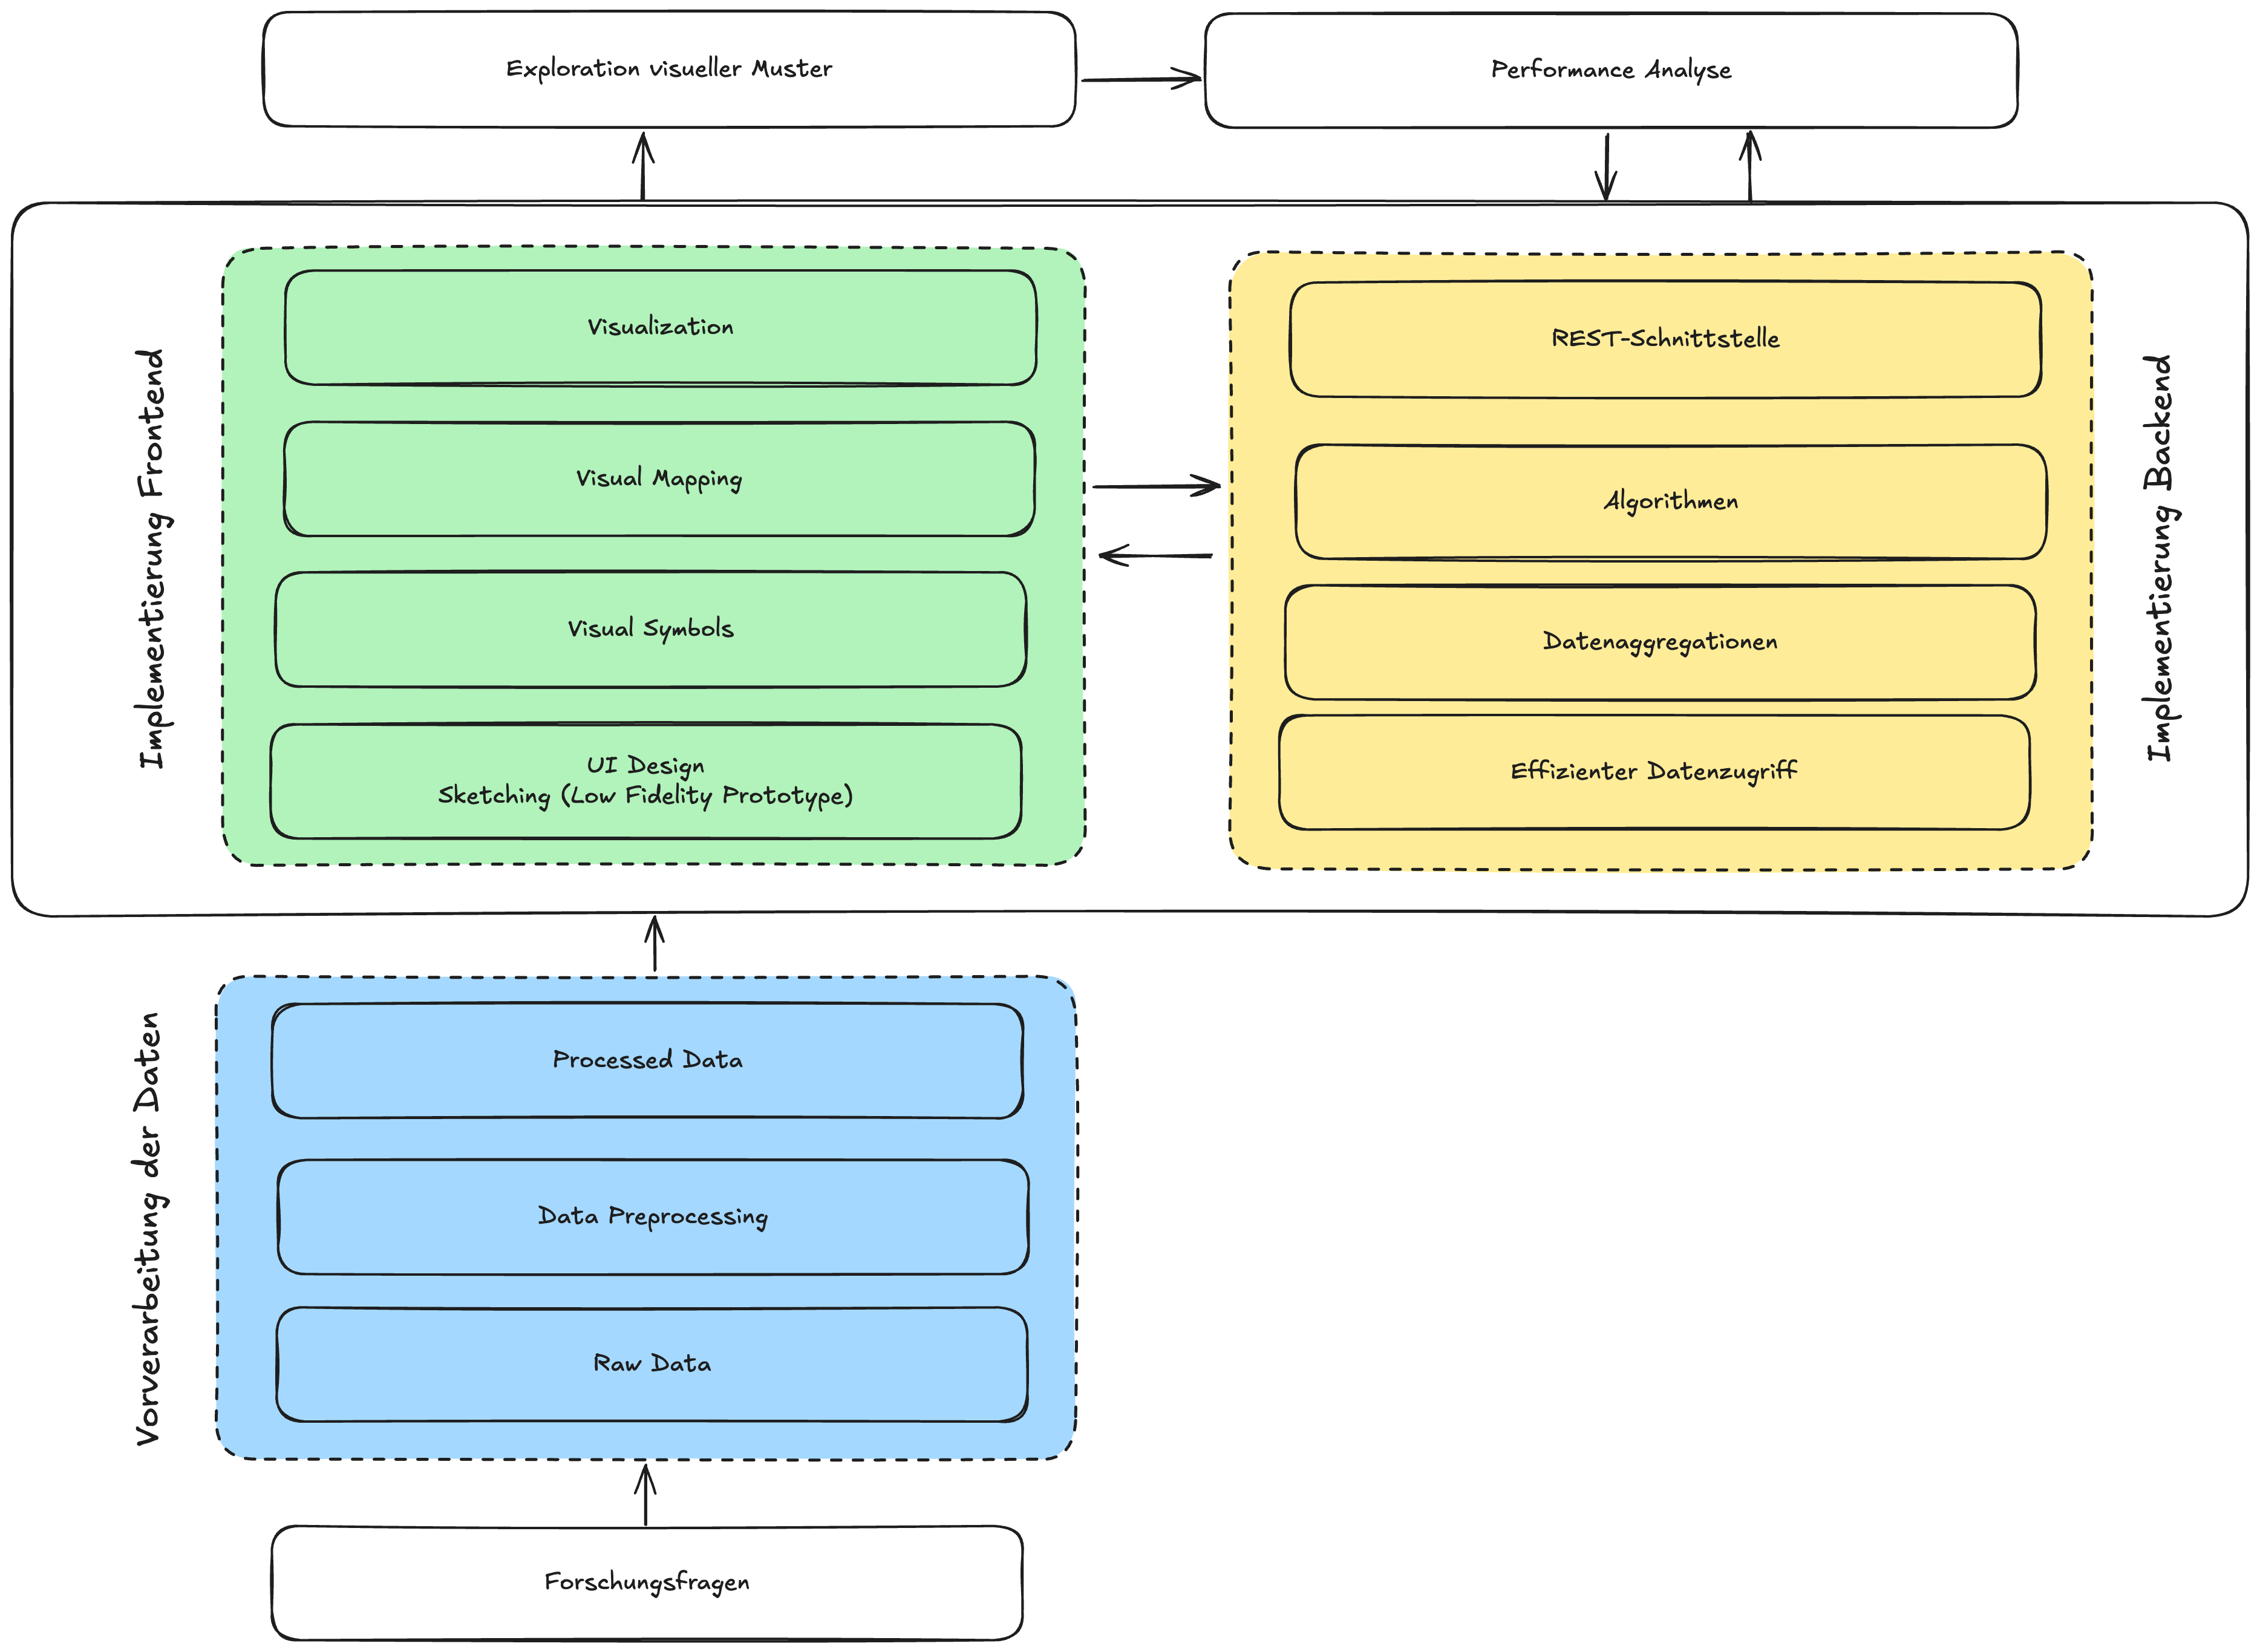
\includegraphics[width=.8\linewidth]{content/00_assets/vorgehen.png}
    \label{fig_vorgehen}
\end{figure}


Das VA-Tool selbst wird aus drei Hauptbestandteilen aufgebaut, einem \textit{Frontend}, einem \textit{Backend}, sowie einer \textit{\acrfull{rest} API}. Das \textbf{Frontend} ist hierbei für die Visualisierung der Daten sowie die Handhabung der Nutzerinteraktionen zuständig. Das \textbf{Backend} ist für die notwendigen Algorithmen und die Datenabfragen verantwortlich. Das Frontend und Backend kommunizieren miteinander über eine  \acrshort{rest} Schnittstelle (siehe Abbildung \ref{fig_va_tool_design}). Diese Trennung hat den Vorteil, dass die Visualisierungslogik von der Anwenderlogik getrennt ist und somit die Visualisierungslogik unabhängig von der Anwendungslogik ausgetauscht werden kann.

\begin{figure}[H]
    \caption{Technischer Aufbau des VA-Tools (eigene Darstellung)}
    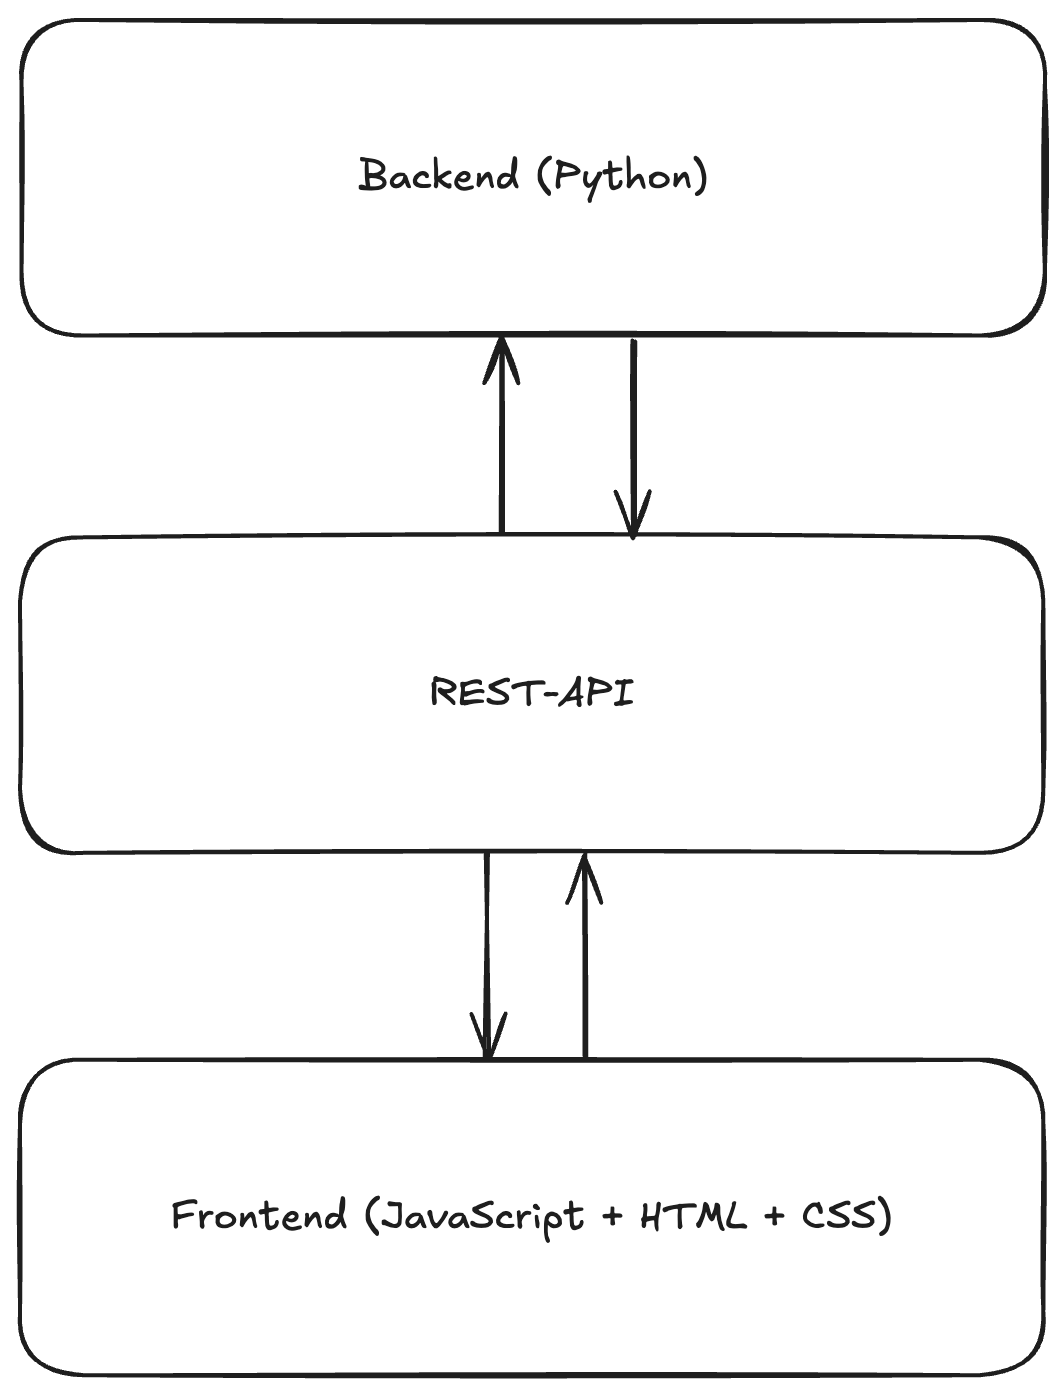
\includegraphics[width=.3\linewidth]{content/00_assets/aufbau_va_tool.png}
    \label{fig_va_tool_design}
\end{figure}

Nachfolgend wird auf die wichtigsten Elemente gemäss Abbildung \ref{fig_vorgehen} eingegangen.

\section{Vorverarbeitung der Daten}
Ausgehend von den Forschungsfragen werden die Datenquellen evaluiert und entsprechend aufbereitet.

\subsection{Raw Data}
Als Datengrundlage dienen die öffentlich zugänglichen Daten der SBB auf Open Data\footnote{\url{https://data.sbb.ch/pages/home/}}. Als Hauptdatenquelle wird die Gegenüberstellung von Zielankunftszeit zu den effektiven Ankunftszeiten verwendet\footnote{\url{https://data.sbb.ch/explore/dataset/actual-data-sbb-previous-day/information/}}. Hieraus lassen sich die Verspätungen pro Station und Zuglinie ermitteln. Als weitere Datenquellen wird das Betriebspunktenetz\footnote{\url{https://data.sbb.ch/explore/dataset/linie-mit-betriebspunkten/information/}} verwendet. Weitere Datenquellen werden im Verlaufe der Arbeit, soweit sinnvoll, hinzugenommen.

\subsection{Data Preprocessing}
Innerhalb des Data Preprocessing werden die Daten optimal zur Beantwortung der Forschungsfragen aufbereitet. Hierunter fallen insbesondere das Data Cleaning sowie evtl. notwendige Daten-Aggregationen. Um sicherzustellen, dass einfach neue Datensätze eingebunden werden können, wird ein entsprechendes Python-Script geschrieben, welches das Data Preprocessing automatisiert.

\subsection{Processed Data}
Die vorverarbeiteten Daten werden optimal für einen schnellen Zugriff gespeichert. Falls notwendig, werden  Datenbanksysteme speziell für analytische Datenauswertungen wie DuckDB verwendet.

\section{Implementierung Frontend und Backend}
Sowohl Frontend und Backend werden parallel entwickelt. Dies ist notwendig um die Daten, welche das Backend liefert, dem Nutzer zu visualisieren, als auch um auf bestimmte Nutzerinteraktionen (Filterung, Anpassung der Parameter) zu reagieren und gegebenenfalls die Algorithmen anzupassen.

\subsection{Frontend}
Ausgehend von den Forschungsfragen sowie den vorverarbeiteten Daten wird ein Low Fidelity Prototyp des VA-Tools in Form einer Skizze erstellt. Aufgrund der Skizze werden anschliessend die Visual Symbols (Liniendiagramme etc.) umgesetzt. Um möglichst viele Endnutzer zu erreichen, wird das Frontend als Web-Applikation mittels JavaScript, HTML und CSS entwickelt.

\subsection{Backend}
Das Backend beinhaltet die komplette Algorithmik und ist für einen effizienten Datenzugriff und entsprechende Datenaggregation notwendig. Bei den Algorithmen werden verschiedene Cluster-Algorithmen evaluiert (bspw. K-Means für räumliches Clustering). Teil des Backends ist auch die Implementierung einer \acrshort{rest} Schnittstelle.

\section{Exploration visueller Muster und Performance Analyse}
Nachdem das Frontend sowie Backend erstellt wurden, können die visuellen Muster mithilfe des VA-Tools exploriert werden. Um eine effiziente Exploration zu ermöglichen, wird auch eine Performance-Analyse durchgeführt, was wiederum Anpassungen am Front- sowie Backend mit sich führen kann.

    \chapter{Meilensteine und Zeitplan}
\label{kap:meilensteine_zeitplan}
Die Meilensteine wurden aufgrund des beschriebenen Vorgehens in Kapitel \ref{kap:forschungsdesign} definiert. Der Hauptteil der Masterarbeit besteht in der Implementierung eines VA-Tools. Anschliessend sollen Trends und Anomalien im Zugnetzwerk der \acrshort{sbb} mithilfe des entwickelten Tools exploriert werden. Für die Entwicklung des VA-Tools sind die Meilensteine M0 bis M2 vorgesehen. Wie bereits in Kapitel \ref{kap:forschungsdesign} erwähnt, wird das VA-Tool als Web-Applikation (Frontend, Backend und \acrshort{rest}-Schnittstelle) umgesetzt. Das Explorieren der Daten mithilfe des Tools erfolgt im Meilenstein M3. Dem Autor ist es zudem wichtig, ein skalierbares VA-Tool zu entwickeln. Dies wird mithilfe des Meilensteins M4 sichergestellt (siehe Tabelle \ref{table:meilensteine}). Eine detaillierte Beschreibung zu den einzelnen Aufgaben pro Meilenstein kann dem Zeitplan im Anhang \ref{attachment:zeitplan} entnommen werden.

\begin{table}[ht]
    \caption{Übersicht der Meilensteine}
    \begin{tabularx}{\textwidth} {
        >{\raggedright\arraybackslash}X 
        >{\raggedright\arraybackslash}X}
            \hline
            \textbf{Meilenstein} & \textbf{Datum} \\
            \hline
            M0: Datenvorverarbeitung     & 18.05.2025     \\
            M1: Implementierung Frontend & 15.06.2025     \\
            M2: Implementierung Backend  & 15.06.2025     \\
            M3: Anwendung VA-Tool        & 29.06.2025     \\
            M4: Performance Analyse      & 13.07.2025     \\
            M5: Abschluss Masterarbeit   & 25.07.2025     \\
            \hline
    \end{tabularx}
    \bigbreak
    \label{table:meilensteine}
\end{table}

    % Ende Textteil
    
    % Start Nachspann
    \printbibliography[heading=bibintoc,title={Literaturverzeichnis}]
    \chapterNoNr{Hilfsmittelverzeichnis}


\begin{table}[ht]
\begin{tabularx}{\textwidth}{
    >{\hsize=.3\hsize\raggedright\arraybackslash}X
    >{\raggedright\arraybackslash}X}
        \hline
            \textbf{Hilfsmittel} & \textbf{Prompts}\\
        \hline
        ChatGPT-4, chat.openai.com & a) «Optimiere den Text nach folgenden Kriterien: …» (23.05.23) \newline b) «Generiere eine SPPS-Syntax für…» (24.04.23)\\
        \hline
        DALL-E, labs.openai.com/  & a) «Impressionalist oil painting of a football player» (12.04.23) \\
        \hline
\end{tabularx}
\end{table}
    \appendix
    \chapter{Einseitiges PDF einbinden}
Es ist möglich, PDF als Grafiken einzubinden. Hier ein Beispiel:
\begin{figure}[H]
    \centering
    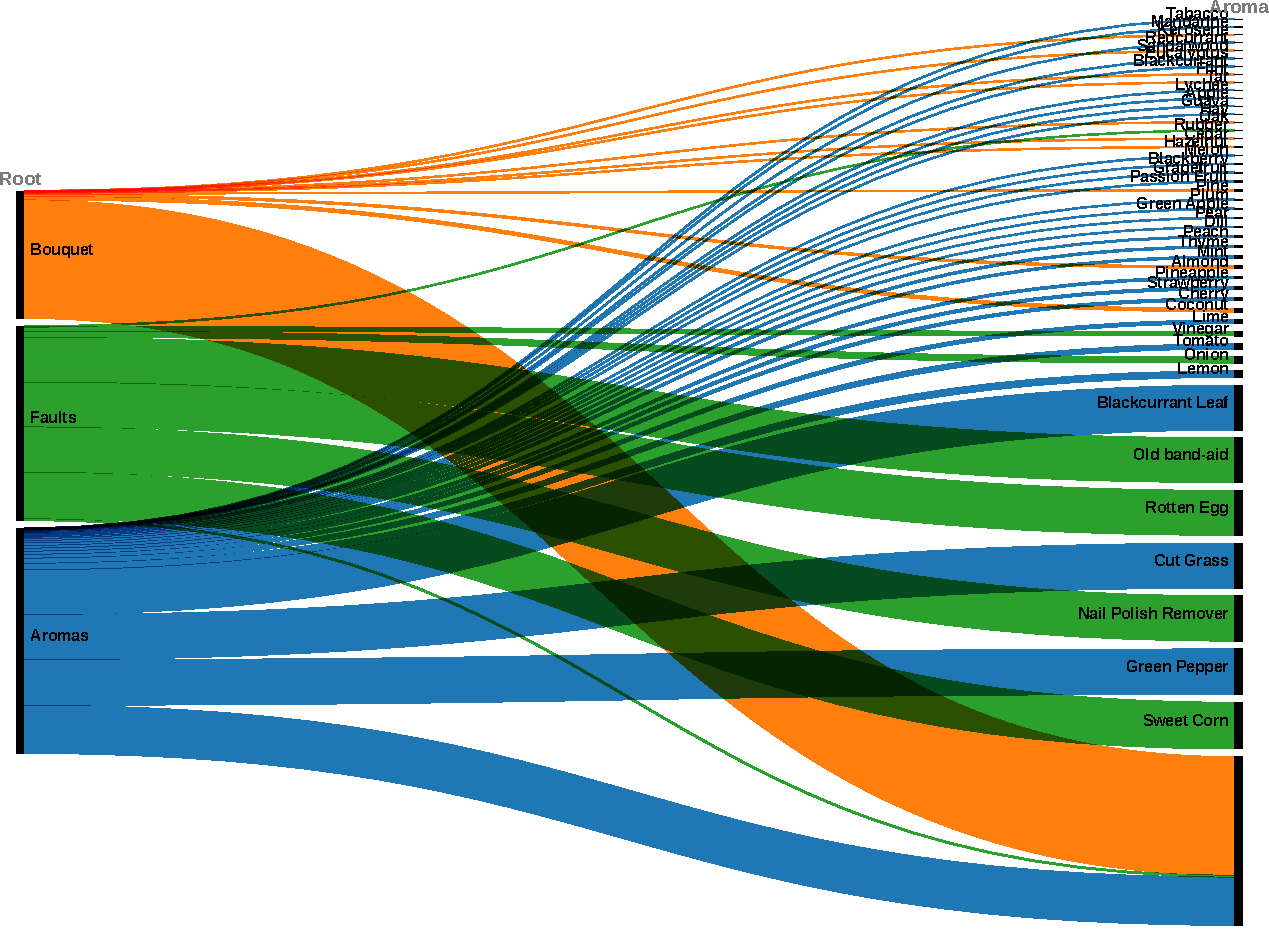
\includegraphics[width=\textwidth]{content/00_assets/example.pdf}
    \caption{Beispiel für Einbindung von PDF-Dateien}
    \label{fig:enter-label}
    \note{Grafik von https://www.rawgraphs.io/}
\end{figure}

\chapter{Mehrseitiges PDF einbinden}
Das Einbinden mehrseitiger PDF ist mittels des \lstinline{pdfpages} Pakets\footnote{https://www.ctan.org/pkg/pdfpages} möglich. Mit dem folgenden Befehl werden die Seiten 9, 15, 25 und 48-50 aus dem books-of-bread PDF eingebunden \parencite{simmons_book_1903}: \\
\lstinline|\includepdf[pages={9,15,25,48-50}]{content/00_assets/book-of-bread.pdf}|

\includepdf[pages={9,15,25,48-50}]{content/00_assets/book-of-bread.pdf}
    \thispagestyle{empty}
\noindent
Ich erkläre hiermit, dass ich diese Arbeit selbstständig verfasst und keine anderen als die angegebenen Quellen und erlaubten Hilfsmittel benutzt habe, einschliesslich der Verwendung von KI-Systemen. Alle Stellen, die wörtlich oder sinngemäss aus Quellen entnommen worden sind, habe ich als solche gekennzeichnet. Ich bin den Vorgaben des Leitfadens wissenschaftliches Arbeiten gefolgt. Mir ist bekannt, dass andernfalls die Hochschulleitung zum Entzug der aufgrund meiner Arbeit verliehenen Qualifikation oder des für meine Arbeit verliehenen Titels berechtigt ist.\\
\\
\\
\\
\ort, \abgabedatum \hfill 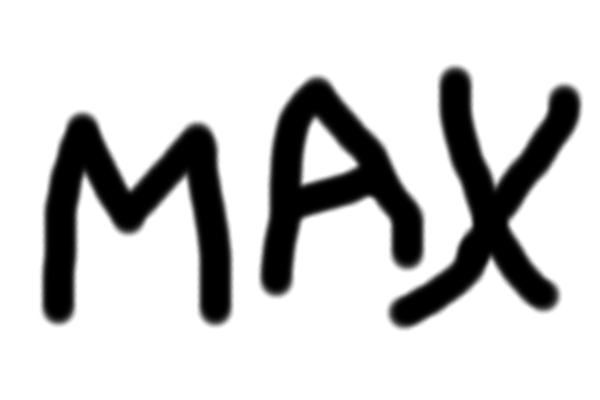
\includegraphics[width=2cm]{content/00_assets/unterschrift.png}\\
Ort, Datum \hfill Unterschrift \autorenschaft

    % Ende Nachspann
    
\end{document}